\documentclass[35pt,landscape]{tikzposter}



\usepackage[utf8]{inputenc}

\usetheme{Basic}

\title{FemtoGraph: A Pregel Based Multithreaded
  Graph Processing Library}

\author{
  \textbf{Alex Ballmer}\\
  \textit{Illinois Institute of Technology}\\
  alexandersballmer@gmail.com\\
  \textbf{Ioan Raicu}\\
  \textit{Illinois Institute of Technology}\\
  iraicu@cs.iit.edu\\
}
\geometry{paperwidth=243.84cm,paperheight=121.92cm}



\begin{document}

\maketitle

\begin{columns}
    \column{0.5}
    \block[roundedcorners=40]{Abstract} {


  The emerging applications for large graphs in big data science and social networks has led to the development of numerous parallel or distributed graph processing applications. The need for faster manipulation of graphs has driven the need to scale accross large core counts and many parallel machines. While distributed memory parallel systems continue to be used for high performance computing, some smaller systems make use of shared memory (SMP) and larger core counts. I hope to explore ways to utilize these larger shared memory systems by implementing a framework for manipulating graphs at a large scale. This system should be able to leverage and scale to very large core counts and provide a framework for later incorporating distributed processing across multiple nodes.
}


    \block[roundedcorners=40]{Implementation} {

      \begin{itemize}
      \item Written in C++ with boost libraries
      \item Graph stored in adjacency list
      \item Message queue based on multiple Boost lockfree queue
      \item Uses normal std::thread for multithreading.
      \end{itemize}


     }
    
    \block[roundedcorners=40]{Final Results} {
      \setcounter{figurecounter}{98}
      \begin{tikzfigure}[Scaling vs GraphLab\label{test_lable}]
        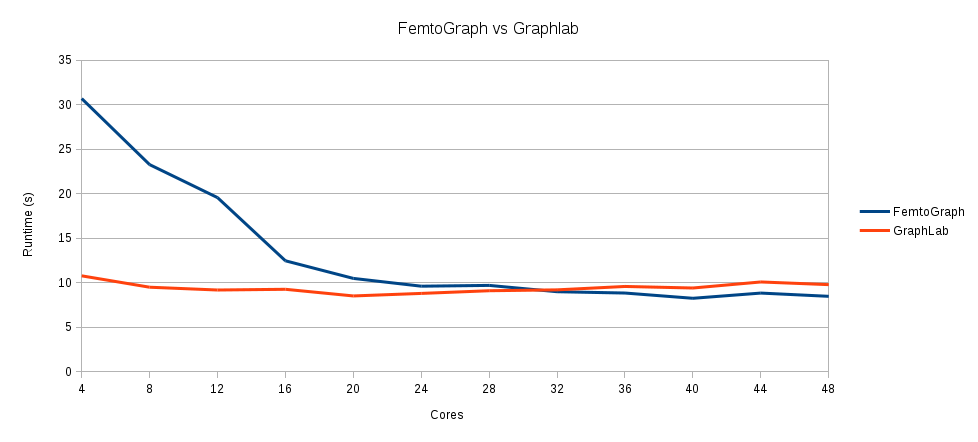
\includegraphics[width=0.95\linewidth]{vs.png}
        \end{tikzfigure}


      }

    
\end{columns}
\end{document}
